\documentclass{article}
\usepackage{tkz-euclide}
\thispagestyle{empty}
\begin{document}
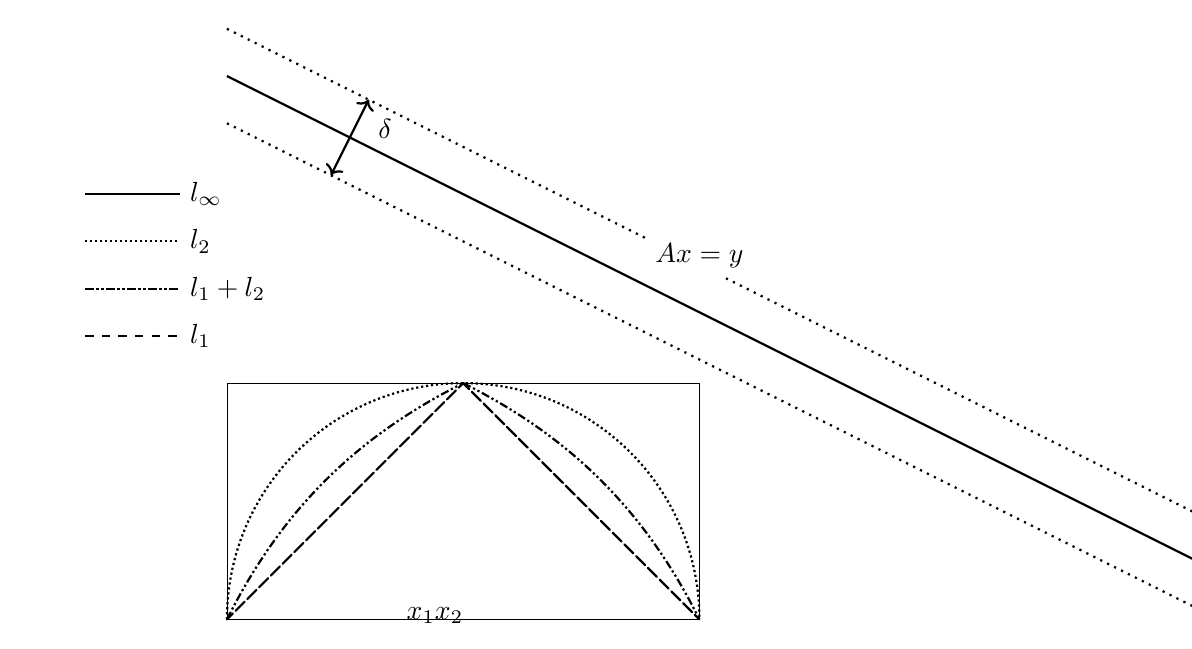
\begin{tikzpicture}[scale=6]
\tkzInit[xmin=-.8,ymin=-.3,xmax=.8,ymax=.8]
\tkzDrawXY[noticks,/tkzdrawX/label=$x_1$,/tkzdrawY/label=$x_2$]

\tkzDefPoint(-1/2, 0){A}
\tkzDefPoint(-1/2, 1/2){B}
\tkzDefPoint( 1/2, 1/2){C}
\tkzDefPoint( 1/2, 0){D}
\tkzDefPoint( 0, 1/2){E}

%% some affine set Ax = y i.e. line
\draw[thick, dotted, scale=1, domain=-1/2:1.6, variable=\x] plot ({\x}, { -0.5*\x + 0.8 });
\draw[thick, scale=1, domain=-1/2:1.6, variable=\x] plot ({\x}, { -0.5*\x + 0.9 });
\draw[thick, dotted, scale=1, domain=-1/2:1.6, variable=\x] plot ({\x}, { -0.5*\x + 1 });

%% l_1 unit norm ball
\tkzDrawPolygon[thick, dashed](A,E)
\tkzDrawPolygon[thick, dashed](E,D)

%% l_1 + l_2
\draw[thick, densely dashdotdotted, scale=1, smooth, domain=-1/2:0, variable=\x] plot ({\x}, { (2*\x + 1) / (2*(\x + 1)) });
\draw[thick, densely dashdotdotted, scale=1, smooth, domain=0:1/2, variable=\x] plot ({\x}, { (2*\x - 1) / (2*(\x - 1)) });

%% l_2 unit norm ball
\draw[thick, densely dotted] (-1/2,0) arc (180:0:1/2);

%% l_infinity unit norm ball
\tkzDrawPolygon(A,B,C,D)

%% legend
\draw[thick] (-.8, .9) -- (-.6, .9) node[right] {$l_{\infty}$};
\draw[thick, densely dotted] (-.8, .8) -- (-.6, .8) node[right] {$l_2$};
\draw[thick, densely dashdotdotted] (-.8, .7) -- (-.6, .7) node[right] {$l_1 + l_2$};
\draw[thick, dashed] (-.8, .6) -- (-.6, .6) node[right] {$l_1$};

%% labels
\draw[thick, <->] (-7/25,47/50) -- (-1/5,11/10);
\node[fill=white] at (1/2,.77) {$Ax = y$};
\node[below right] at (-0.2,1.08) {$\delta$};

\end{tikzpicture}
\end{document}